\Chapter{A fejlesztőkörnyezet implementációja}

\graphicspath{{./kepek/}}

\Section{Minimális program: egy fájlt kezelő kódszerkesztő}

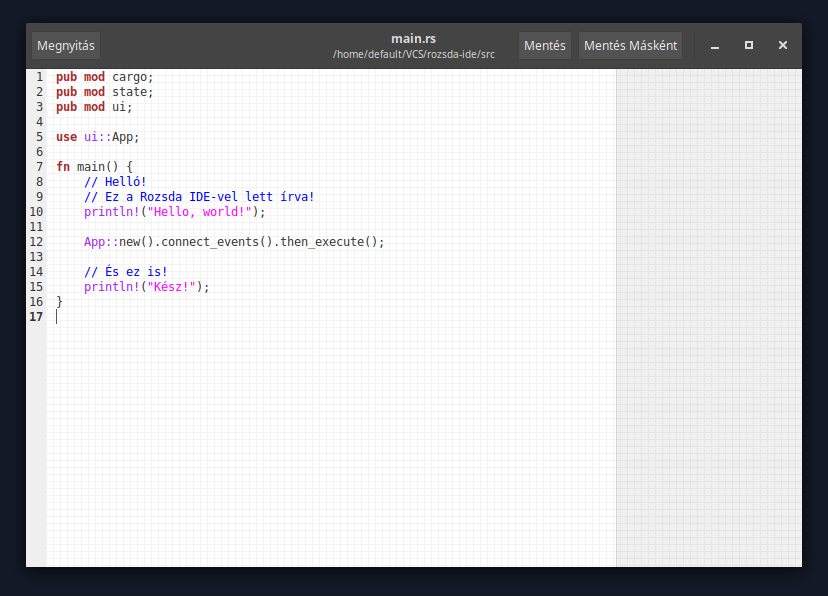
\includegraphics[width=\textwidth]{program-mvp}

A program implementációját egy olyan minimális életképes termék elkészítésével kezdjük,
ami meg tud nyitni egyszerre egy fájlt, annak tartalmát megfelelően dekorálja,
ha az egy Rust forráskód-fájl, és tud az eredeti, vagy egy másik megadott fájlba menteni.

A programnak ez a része Michael Murphy \textit{Simple Common Mark Editor} projektjén alapul.\cite{gtk_tutorial}
Murphy programra Markdown formátumú fájlokat kezel, illetve azokat HTML formátumra lefordítja,
és megjeleníti a felhasználónak.
A leglényegesebb változtatások ezen a programon a Markdown nyelv lecserélése a Rust nyelvre,
a projekt frissítése egyrészt a Rust 2018-as verziójára, illetve a függőségek frissítése a legújabb verziókra.

A projekt egy \texttt{cargo new} parancshívással kezdődik.

% TODO:
% - Megnyitás, mentés
% - ActiveMetadata
% - FileChooserDialog
% - események csatlakoztatása App-ban
% - Main

% TODO: Részletesen be kell mutatni a tervezést és az implementációt!

% Lehet hozzá jó sok ábra. Az implementációnál itt szerepelhetnek kódrészletek.